%\begin{tcolorbox}[title=TODO]
%Measurement results / analysis / discussion: 1/3
%\begin{itemize}
%\item whatever you have done, you must comment it, compare it to other systems, evaluate it
%\item usually, adequate graphs help to show the benefits of your approach
%\item caution: each result/graph must be discussed! what's the reason for this peak or why have you ovserved this effect
%\end{itemize}
%\end{tcolorbox}

\section{Image Size}
It has been possible to create a minimal \ac{OS} image with the Azure IoT Edge runtime
using \textit{reUpNix}. To achieve this, \textit{Nix} derivations and modules for
the \textit{Azure IoT Edge} runtime and the \textit{Azure IoT Edge Identity Service}
have been created. Additionally, a \textit{Nix} derivation for the \ac{ADU} Agent has been created.
Microsoft has the source code for the previously mentioned components
publicly available on GitHub, the \textit{Nix} packages could be built directly
from source code, which is written in Rust and C and uses Cargo and CMake respectively.
For the third-party dependencies, namely \textit{libc}, \textit{libtss}, \textit{libcurl}, and
\textit{openssl}, of the \textit{Azure IoT Edge} runtime, the already existing \textit{Nix} packages
from the \textit{Nixpkgs} repository have been used.
By using the existing \textit{Nix} packages, it could be ensured that the dependencies
are linked with the correct paths in the \textit{Nix} store and can be reused
by other \textit{Nix} packages.
Further, the already existing \textit{Nix} package for \textit{Docker} had to be added
to the system configuration, since it is required by \textit{Azure IoT Edge}.
However, it is not a hard dependency, in case the user wants to exchange \textit{Docker}
with \textit{Moby} or \textit{Podman}, which are also able to run \ac{OCI}-compliant
container images. \textit{Podman} in particular might even further reduce, the
image size (see section \ref{sec:podman}).

Finally, since \textit{reUpNix} removes some unnecessary
Kernel modules, Kernel modules had to be added back to the system configuration in order
to be able to run \textit{Docker}.
Most notably, the kernel modules
\textit{br\_netfilter}, \textit{xt\_nat} and \textit{8021q} had to be added to the system configuration,
since they are required for \textit{Docker} networking.

\textit{reUpNix}, \textit{NixOS 23.01}, \textit{Ubuntu 22.04}, and
\textit{Yocto Kirkstone} had to be compared by their installed image size, with the methodology introduced
in chapter \ref{sec:image-size}. All system images feature an \ac{OCI}-compliant container runtime
and the Azure IoT Edge runtime. The results of the comparison are shown in table \ref{tab:image-size}.

\clearpage

\begin{table}[H]
	\centering
	\begin{tabular}{l|l|l}
	\toprule
		Operating System & Image Size & $\Delta$ Ubuntu\\
	\midrule
    \textbf{reUpNix} & \text{1 289 MB} & \color{ba-green}{- 1 010 MB} \\
    \textbf{NixOS 23.01} & \text{2 361 MB} & \textcolor{ba-red}{+ 62 MB} \\
    \textbf{Ubuntu 22.04} & \text{2 299 MB} & \text{-} \\
    \textbf{Yocto Kirkstone} & \text{4 933 MB} & \textcolor{ba-red}{+ 2 634 MB} \\
	\bottomrule
	\end{tabular}
	\caption{Image size by OS for each variation}
	\label{tab:image-size}
\end{table}

\noindent
It can be seen from table \ref{tab:image-size} that with its 1,289 \ac{MB},
\textit{reUpNix} has a 43\% smaller base image size than Microsoft's recommended
\textit{Ubuntu 22.04}. It is also 45\% smaller than the base image size of
\textit{NixOS 23.01}, which shows that the minification process is very effective
in minimizing the size of the \ac{OS} on disk despite having a fully working
Azure IoT Edge runtime installed.
To further illustrate the differences in size, refer to figure \ref{fig:image-size}.


\begin{figure}[htbp]
  \centering
  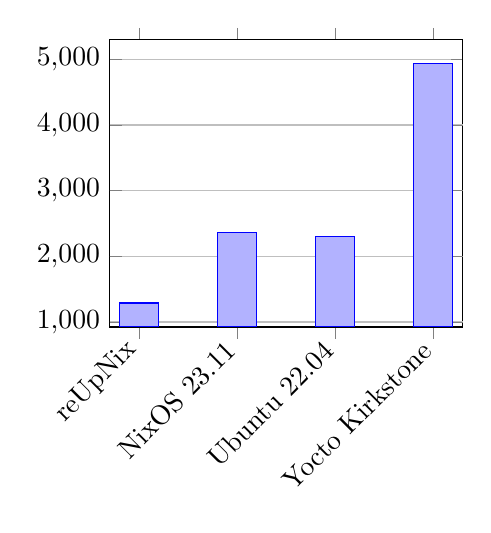
\begin{tikzpicture}
    \begin{axis}[
      ybar,
      bar width=0.5cm,
      width=0.5\textwidth,
      % height=0.5\textwidth,
      xtick=data,
      xticklabels={
        {reUpNix},
        {NixOS 23.11},
        {Ubuntu 22.04},
        {Yocto Kirkstone}
      },
      x tick label style={rotate=45,anchor=east}, % Rotating labels
      ymajorgrids=true, % Major grid lines for y-axis
      ytick={0,1000,2000,3000,4000,5000}, % Y-axis tick marks
      extra y ticks={1000,2000,3000,4000}, % Additional y-axis tick marks
      extra y tick labels={}, % Remove labels for the extra ticks
      ]

      \addplot coordinates {
        (1,1289)
        (2,2361)
        (3,2299)
        (4,4933)
      };

    \end{axis}
  \end{tikzpicture}
\caption{Image size by OS in Megabytes}
\label{fig:image-size}
\end{figure}

\noindent
On the contrary, the difference in image size between \textit{Ubuntu 22.04} and
\textit{NixOS} is only 62 Megabytes, which is unsurprising, since both are
general purpose \textit{Linux} distributions and not specifically designed
for embedded and \ac{IoT} systems. The largest image in this comparison is
\textit{Yocto Kirkstone}, which is 2,634 Megabytes larger than \textit{Ubuntu 22.04}.
However, it features no effort to minimize the size of the \ac{OS} and it
just contains a default development configuration of the \textit{Yocto Project}
for \textit{Azure IoT Edge}. It can be seen that the hypothesis, that \textit{reUpNix}
is by far the smallest \ac{OS} in this comparison, is confirmed. The minification
process is effective and \textit{reUpNix} is a viable option for \ac{IoT} devices
running \textit{Azure IoT Edge} with limited storage capacity. Even if it would be
updated \textit{reUpNix} with an A/B partitioning scheme, which is not the proposed
methodology, the update size would be smaller, and it would still have less data
transmitted in comparison to the other \ac{OS}.

\subsection{Podman}
\label{sec:podman}
Podman is a container runtime developed by Red Hat and a direct competitor to Docker.
In the future, it would be interesting to investigate the possibility of using
Podman instead of Docker as the container runtime for Azure IoT Edge. Podman is
not officially supported by Microsoft, but it can potentially be used as a
replacement for Docker since it can provide a \ac{UDS} for the IoT Edge runtime
to communicate with the container runtime \cite{book:3556946,msdoc-supportetplatforms}.
In a quick comparison made with an unminified \textit{NixOS} image, it has been found that
using \textit{Podman} instead of \textit{Docker} would reduce the image size by
15\%. However, \textit{Podman} does not run on \textit{reUpNix} out of the box.
Some effort to investigate, which components have to be
added to \textit{reUpNix} be able to run \textit{Podman}, would have to be invested.

\section{Update size}
In the previous section, it has already been discussed that it has been possible to create
\textit{Nix} packages for the \textit{Azure IoT Edge} runtime and its dependencies.
Since it has been established that \textit{reUpNix} can be used to create a minimal
\ac{OS} image for \textit{Azure IoT Edge}, the update size when updating with \textit{reUpNix}'s differential updates
can now be compared to the update size when updating in an A/B partitioning scheme.
Both methods can be used with \ac{ADU} Agent, with the exception that for \textit{reUpNix} the \ac{ADU}
needs to use a script handler to apply the update, while for A/B partitioning
the built-in \ac{ADU} handler can be used. When comparing the update size
for an update, which changes the majority of packages in the system, a \textit{Nixpkgs} version from November 1st, 2023 as the base and March 16th, 2024 as the target upstream have been picked. The results of the comparison are shown in table
\ref{tab:update-size}.

\begin{table}[H]
	\centering
	\begin{tabular}{l|l|l}
	\toprule
		Operating System & Image Size & $\Delta$ Ubuntu\\
	\midrule
    \textbf{reUpNix} & \text{206 MB} & \color{ba-green}{- 1 928 MB} \\
    \textbf{Ubuntu 22.04} & \text{2 134 MB} & \text{-} \\
    \textbf{Yocto Kirkstone} & \text{4 717 MB} & \textcolor{ba-red}{+ 2 583 MB} \\
	\bottomrule
	\end{tabular}
	\caption{Update size by OS for each variation}
  \label{tab:update-size}
\end{table}

\noindent
It can be clearly seen that \textit{reUpNix} has a 90.3\% smaller update size
than \textit{Ubuntu 22.04}, which is a significant improvement. Applying the
differential update methodology of \textit{reUpNix} to \ac{IoT} devices
running \textit{Azure IoT Edge} will significantly reduce the amount of data
transmitted in comparison to using A/B partitioning. This is important for
devices with a limited Internet connection and it enables a more frequent updating.

\begin{figure}[htbp]
  \centering
  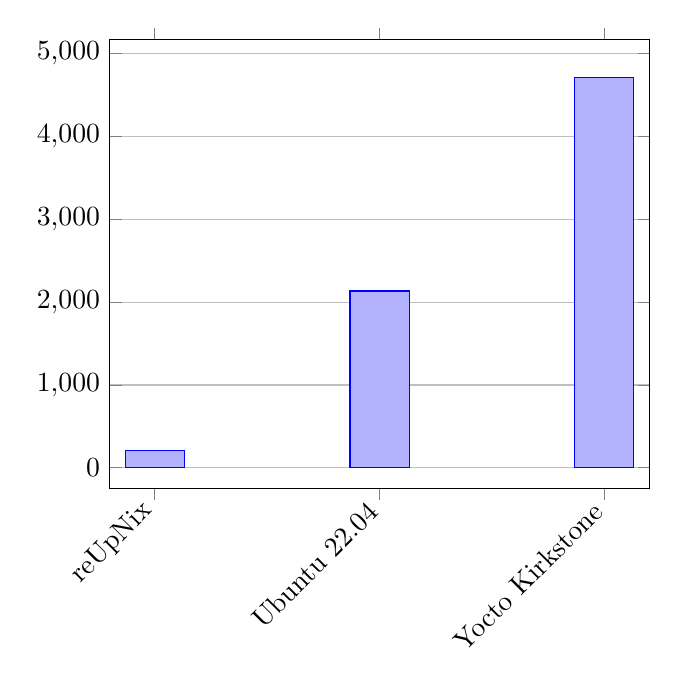
\begin{tikzpicture}
    \begin{axis}[
      ybar,
      bar width=0.75cm,
      % width=0.5\textwidth,
      % height=0.5\textwidth,
      xtick=data,
      xticklabels={
        {reUpNix},
        {Ubuntu 22.04},
        {Yocto Kirkstone}
      },
      x tick label style={rotate=45,anchor=east}, % Rotating labels
      ymajorgrids=true, % Major grid lines for y-axis
      ytick={0,1000,2000,3000,4000,5000}, % Y-axis tick marks
      extra y ticks={1000,2000,3000,4000}, % Additional y-axis tick marks
      extra y tick labels={}, % Remove labels for the extra ticks
      ]

      \addplot coordinates {
        (1,206)
        (2,2134)
        (3,4717)
      };

    \end{axis}
  \end{tikzpicture}
\caption{Update Size by OS in Megabytes}
\label{fig:update-size}
\end{figure}

\noindent
In figure \ref{fig:update-size} it can be seen yet again how large the difference
in size is and that \textit{reUpNix} is the most efficient \ac{OS} in this comparison.
Using \textit{reUpNix} for \ac{IoT} devices running \textit{Azure IoT Edge}
instead of Microsoft's recommended \textit{Ubuntu 22.04} will significantly reduce
the data transmitted, when updating the \ac{OS} and the \textit{Azure IoT Edge} runtime.

\section{Time To Recover}
In order to verify that the \textit{reUpNix} system can recover from a reboot
in an acceptable time frame, the time it takes for the system to
reboot and send a message via the \textit{Azure IoT Edge Hub} with the proposed
methodology from chapter \ref{sec:time-to-recover} has been measured. The first message
that the \textit{Edge Agent} sends to the \textit{Edge Hub} after a reboot as
a measure has been used, because this message includes the timestamp when it was sent.
The \textit{Edge Agent} immediately sends an update message to the \textit{Azure
IoT Hub} to signal that the device is online. The same experiment has been repeated
for all of the \ac{OS}, namely \textit{reUpNix}, \textit{NixOS 23.01},
\textit{Ubuntu 22.04}, and \textit{Yocto Kirkstone}. The results of the comparison
can be seen in table \ref{tab:timetorecover} and figure \ref{fig:timetorecover}.


\begin{table}[H]
	\centering
	\begin{tabular}{l|l|l|l|l}
	\toprule
		Operating System & Average & Adjusted Average\footnote &  Std. Deviation & Std. Error \\
	\midrule
    \textbf{reUpNix} & 16.0 & 15.0 &  2.44 & 0.67 \\
    \textbf{NixOS 23.01} & 24.06 & 19.06 & 8.73 & 1.62 \\
    \textbf{Ubuntu 22.04} & 33.30 & 23.30 & 8.74 & 1.82 \\
    \textbf{Yocto Kirkstone} & 260.71 & 250.71 & 10.39  & 2.77 \\
	\bottomrule
	\end{tabular}
	\caption{Average Time to Recover by OS in Seconds}
	\label{tab:timetorecover}
\end{table}
\footnotetext{The adjusted average accounts for the delay that is configured in
the bootloader to wait for user input, which is 1 second for \textit{reUpNix},
5 seconds for \textit{NixOS 23.01}, and 10 seconds for \textit{Yocto Kirkstone}
and \textit{Ubuntu 22.04} respectively.}

\begin{figure}[H]
\centering
\begin{tikzpicture}
  \begin{axis}[
    title  = ReUpNix,
    ybar,
    bar width=0.05cm,
    enlarge y limits  = {0.15,upper},
    width = 0.3\textwidth,
  ]
    \addplot table [x=seconds, y=times, col sep=comma] {data/time-to-recover-reupnix.csv};
    \draw[dashed,red] (axis cs:15.33,\pgfkeysvalueof{/pgfplots/ymin}) -- (axis cs:15.33,\pgfkeysvalueof{/pgfplots/ymax});
    \draw[dashed] (axis cs:16,\pgfkeysvalueof{/pgfplots/ymin}) -- (axis cs:16,\pgfkeysvalueof{/pgfplots/ymax});
    \draw[dashed,red] (axis cs:16.67,\pgfkeysvalueof{/pgfplots/ymin}) -- (axis cs:16.67,\pgfkeysvalueof{/pgfplots/ymax});
  \end{axis}
\end{tikzpicture}
\begin{tikzpicture}
  \begin{axis}[
    title  = NixOS 23.01,
    ybar,
    bar width=0.05cm,
    enlarge y limits  = {0.15,upper},
    width = 0.3\textwidth,
    % nodes near coords,
  ]
    \addplot table [x=seconds, y=times, col sep=comma] {data/time-to-recover-nixos.csv};
    \draw[dashed,red] (axis cs:22.44,\pgfkeysvalueof{/pgfplots/ymin}) -- (axis cs:22.44,\pgfkeysvalueof{/pgfplots/ymax});
    \draw[dashed] (axis cs:24.06,\pgfkeysvalueof{/pgfplots/ymin}) -- (axis cs:24.06,\pgfkeysvalueof{/pgfplots/ymax});
    \draw[dashed,red] (axis cs:25.68,\pgfkeysvalueof{/pgfplots/ymin}) -- (axis cs:25.68,\pgfkeysvalueof{/pgfplots/ymax});
  \end{axis}
\end{tikzpicture}
\begin{tikzpicture}
  \begin{axis}[
    title  = Ubuntu 22.04,
    ybar,
    bar width=0.05cm,
    enlarge y limits  = {0.15,upper},
    width = 0.3\textwidth,
  ]
    \addplot table [x=seconds, y=times, col sep=comma] {data/time-to-recover-ubuntu.csv};

    \draw[dashed,red] (axis cs:31.48,\pgfkeysvalueof{/pgfplots/ymin}) -- (axis cs:31.48,\pgfkeysvalueof{/pgfplots/ymax});
    \draw[dashed] (axis cs:33.3,\pgfkeysvalueof{/pgfplots/ymin}) -- (axis cs:33.3,\pgfkeysvalueof{/pgfplots/ymax});
    \draw[dashed,red] (axis cs:35.12,\pgfkeysvalueof{/pgfplots/ymin}) -- (axis cs:35.12,\pgfkeysvalueof{/pgfplots/ymax});
  \end{axis}
\end{tikzpicture}
\begin{tikzpicture}
  \begin{axis}[
    title  = Yocto Kirkstone,
    ybar,
    enlarge y limits  = {0.15,upper},
    width = 0.3\textwidth,
    bar width=0.05cm,
  ]
    \addplot table [x=seconds, y=times, col sep=comma] {data/time-to-recover-yocto.csv};
    \draw[dashed,red] (axis cs:257.94,\pgfkeysvalueof{/pgfplots/ymin}) -- (axis cs:257.94,\pgfkeysvalueof{/pgfplots/ymax});
    \draw[dashed] (axis cs:260.71,\pgfkeysvalueof{/pgfplots/ymin}) -- (axis cs:260.71,\pgfkeysvalueof{/pgfplots/ymax});
    \draw[dashed,red] (axis cs:263.48,\pgfkeysvalueof{/pgfplots/ymin}) -- (axis cs:263.48,\pgfkeysvalueof{/pgfplots/ymax});
  \end{axis}
\end{tikzpicture}
\caption{Number of Measurements by Duration}
\label{fig:timetorecover}
\end{figure}
\noindent
It can be seen from the results that \textit{reUpNix} has on average the fastest time
to recover, from the four \ac{OS} that have been tested, even when accounting for the different
delays that are configured for the bootloader. So the hypothesis, that \textit{reUpNix}
and \textit{NixOS} will provide no significant delay in the boot process due to
the \textit{Nix} package manager, is confirmed. The two \ac{OS} using the
\textit{Nix} package manager have a similar or better, time to recover as the \ac{OS},
which use a traditional file system and directory structure, even when taking
the standard deviation and standard error into account. Some outliers
for \textit{Ubuntu 22.04} and \textit{NixOS 23.01} have been observed, which are due to the
fact that the reboot command was issued without the force flag, which will cause
the system to wait until all processes are terminated before rebooting. Further,
it can be seen that \textit{reUpNix} has a faster time to recover than \textit{NixOS 23.01},
which means that the minification process of \textit{reUpNix} does not introduce
delay in the boot process and the opposite is true.
The measurements show that \textit{reUpNix} is a viable option for \ac{IoT} devices
and that the \textit{Nix} package manager does not introduce a significant delay.
\textit{Azure IoT Edge} with its dependencies can be installed and run on
\textit{reUpNix} with a comparable, even better, time to recover as Microsoft's
recommended \textit{Ubuntu 22.04}.



\section{Container Updates}
With the proposed methodology in chapter \ref{sec:container-updates}, it has been possible
to install \ac{OCI}-container images on an \ac{IoT} device running \textit{reUpNix} without
using \code{docker pull}. It has been verified that the installed images can be used
to run with \textit{Docker} and \textit{Azure IoT Edge}.
However, due to the \textit{Nix store}
not preserving timestamps and order of files,
the reconstructed image does not have the same \textit{SHA256} checksum as the
original image from \textit{Docker Hub}, but the files are identical. For
\textit{Azure IoT Edge} this is not a problem, since the \textit{Edge Agent} only
references the image by its name and tag and not by its \textit{SHA256} checksum.

To measure the efficiency of the \textit{reUpNix} differential update mechanism
when updating container images, a selection of the most popular container images
from \textit{Docker hub} were updated to the latest version from the previous version
using the \textit{reUpNix} differential update mechanism. \textit{Docker} uses
\textit{gzip} to compress the layers of the image when pulling. For the differential
updates of \textit{reUpNix}, \textit{gzip} was also used to compress the updates,
however, the update can be compressed with any compression algorithm.
The results of the
comparison can be seen in table \ref{tab:container-update-size}.

\begin{table}[H]
	\centering
  \footnotesize
	\begin{tabular}{l|c|c|c|c|c|c}
	\toprule
	 Image & From& To & Layers & Pull Size & reUpNix Size &$\Delta$ \% \\
	\midrule
    \textbf{ubuntu} & jammy-20240212 & jammy-20240227 & 1 & 29.54 MB &28.72 MB & \color{ba-green}{- 2.77 \%} \\
    \textbf{node} & 20.12.0-bullseye & 21.7.1-bullseye & 13 & 357.03 MB & 362.64 MB & \color{ba-red}{+ 1.57 \%} \\
    \textbf{ruby} & 3.1.4-bookworm & 3.2.3-bookworm & 16 & 365.76 MB & 372.82 MB & \color{ba-red}{+ 1.93 \%} \\
    \textbf{busybox} & 1.35.0-glibc & 1.36.1-glibc & 1 & 2.05 MB & 2.15 MB & \color{ba-red}{+ 4.87 \%} \\
	\bottomrule
	\end{tabular}
	\caption{Container Image Update Size}
	\label{tab:container-update-size}
\end{table}

\noindent
The results show that when using the \textit{reUpNix} differential update mechanism
to update container images, the size of the update is slightly larger than the size
when using \code{docker pull} for most of the tested images. This is mostly due
to the fact that when vendors
publish new versions of their container images, they usually include new features
and update the software in the image, which means that almost all files on all
layers have to be updated. The additional size can be explained by the fact that the
\textit{reUpNix}
differential update mechanism takes up some space for the update script itself,
which needs to store information about \textit{Nix store} paths were the files
to update are located. With all the layers unpacked, the paths of the files
in the \textit{Nix store} are quite long, because they include the hash of the
\textit{Nix store} object and are referenced over and over again in the update script,
because of the large number of files.

The established hypothesis, that the \textit{reUpNix} differential update mechanism
are more efficient than using \code{docker pull} for updating container images
is not true. There are however images, like \textit{ubuntu}, where the update size
was smaller when updating with \textit{reUpNix}, but this was mainly due to the
fact that the time between releases was the shortest for this image. However,
in an ideal scenario, where only a few files have changed in an otherwise large layer,
\textit{reUpNix}'s differential update mechanism would be more efficient than
pulling the whole layer.

\subsection{Improved Compression}
To further reduce the update size, the \textit{reUpNix} differential updates can
be compressed with a more efficient algorithm than \textit{gzip}. With \textit{reUpNix}
updates, users are not bound to \textit{gzip}, like with docker. A quick test
yielded that using \textit{bzip2} to compress the updates instead of \textit{gzip},
the update size can be further reduced. For example, the container image \textit{ubuntu}
was 6.3\% smaller when compressed with \textit{bzip2} instead of \textit{gzip}.
